\documentclass{beamer}
\usepackage{ctex} %注意这个宏包
\usepackage{color}
\usepackage{graphics,graphicx}
\usepackage{pstricks,pst-node,pst-tree}
\usetheme{Boadilla}
\usecolortheme{beaver}
\usepackage{pstricks}
\usepackage{pst-plot}
\CTEXoptions[today=old]
\setCJKmainfont[BoldFont={SimHei},ItalicFont={KaiTi}] {WenQuanYi Micro Hei Mono}
\title{Learning HMM Structure for Information Extraction}
\author{Speaker:\\Chunwei Yan}
\institute[PKUSZ]{
    互联网研发中心\\
}
\date{\today}

\begin{document}
% ------------- title page ----------------------------
%--- the titlepage frame -------------------------%
\begin{frame}
  \titlepage
\end{frame}

\section{Begin}
\begin{frame}
\frametitle{Outline}
\tableofcontents
\end{frame}

\section{HMM基础}
\begin{frame}{Introduction to HMM}
\begin{block}{HMM组成 }
    \begin{itemize}
        \item 状态集合 Q \{$q_I, q_0, q_1, \cdots q_F$\}
        \item 状态间的转移 $(q \rightarrow q')$
        \item 一个有限的观测集合 $\sum = \{ \sigma_1, \sigma_2, \cdots, \sigma_M\}$
    \end{itemize}
\end{block}

\begin{block}{模型系数}
\begin{itemize}
    \item 状态转移概率: $P(q \rightarrow q')$
    \item 状态$q$观测为$\sigma$的概率: $P(q \uparrow \sigma)$ 
\end{itemize}
\end{block}
\end{frame}

\begin{frame}{HMM 的使用}
    一个HMM模型观测为一个字符串$x$的概率是:
    \begin{equation}
    P(x|M) = \sum_{q_1,\cdots,q_l \in Q^t} {
        \prod_{k=1}^{l+1}{
            P(q_{k-1} \rightarrow q_k) P(q_k \uparrow x_k)
        }
    }
    \end{equation}
    如下恢复出最可能生成观测$y$的状态序列:
    %To recover the state sequence $V(x|M)$ that has the highest probability of having produced an observation sequence y:
    \begin{equation}
    P(x|M) = \sum_{q_1,\cdots,q_l \in Q^t} {
        \prod_{k=1}^{l+1}{
            P(q_{k-1} \rightarrow q_k) P(q_k \uparrow x_k)
        }
    }
    \end{equation}
\end{frame}

\begin{frame}{ 从科技论文头部挖掘信息}
    %Information Extraction from Research Paper Headers}
    \begin{block}{模型参数学习}
        %Learn Model Parameters}
        可以的两种情况:
        \begin{itemize}
            \item 每一个状态与代表一钟类别,比如 \textbf{标题}, \textbf{作者}, \textbf{地址}等。
            \item 一种类别联系到多种状态,每个状态间仅有有限的转移。
        \end{itemize}
    \end{block}
    
    \begin{block}{ 标注新的论文头部}
        \begin{itemize}
            \item 将论文头部的词作为观测值
            \item 用 \textbf{Viterbi 算法}恢复最有可能的状态序列
        \end{itemize}
    \end{block}
\end{frame}

\section{从训练集中学习HMM模型}
\begin{frame}{Introduction}
    \textbf{首先要确定模型中有多少状态.}
    \begin{block}{可取方案:}
        \begin{itemize}
            \item 仅仅为每一个状态分配一种类别
            \item 将一种类别联系到多个状态
        \end{itemize}
    \end{block}
\end{frame}

% contents 
\begin{frame}{模型学习过程}
    \begin{enumerate}
        \item 为每一个词独立分配一个状态
        \item neighbor-merging(相邻合并)
        \item 进一步合并
            \begin{itemize}
                \item V-merging
                \item M-merging
                \item Bayesian model merging
            \end{itemize}
    \end{enumerate}
\end{frame}

\begin{frame}{模型学习过程}
    \begin{enumerate}
        \item \textbf{\textcolor{red}{为每一个词独立分配一个状态}}
        \item neighbor-merging(相邻合并)
        \item 进一步合并
            \begin{itemize}
                \item V-merging
                \item M-merging
                \item Bayesian model merging
            \end{itemize}
    \end{enumerate}
\end{frame}

\begin{frame}{为每一个词独立分配一个状态}
    为训练集中每一个词分配一个独立的状态,同时,当前词汇与下一个词汇间对应着状态转移
    %Each word in the training data is assignd its own state, which transitions to the state of the word that follows it.
    \begin{center}
        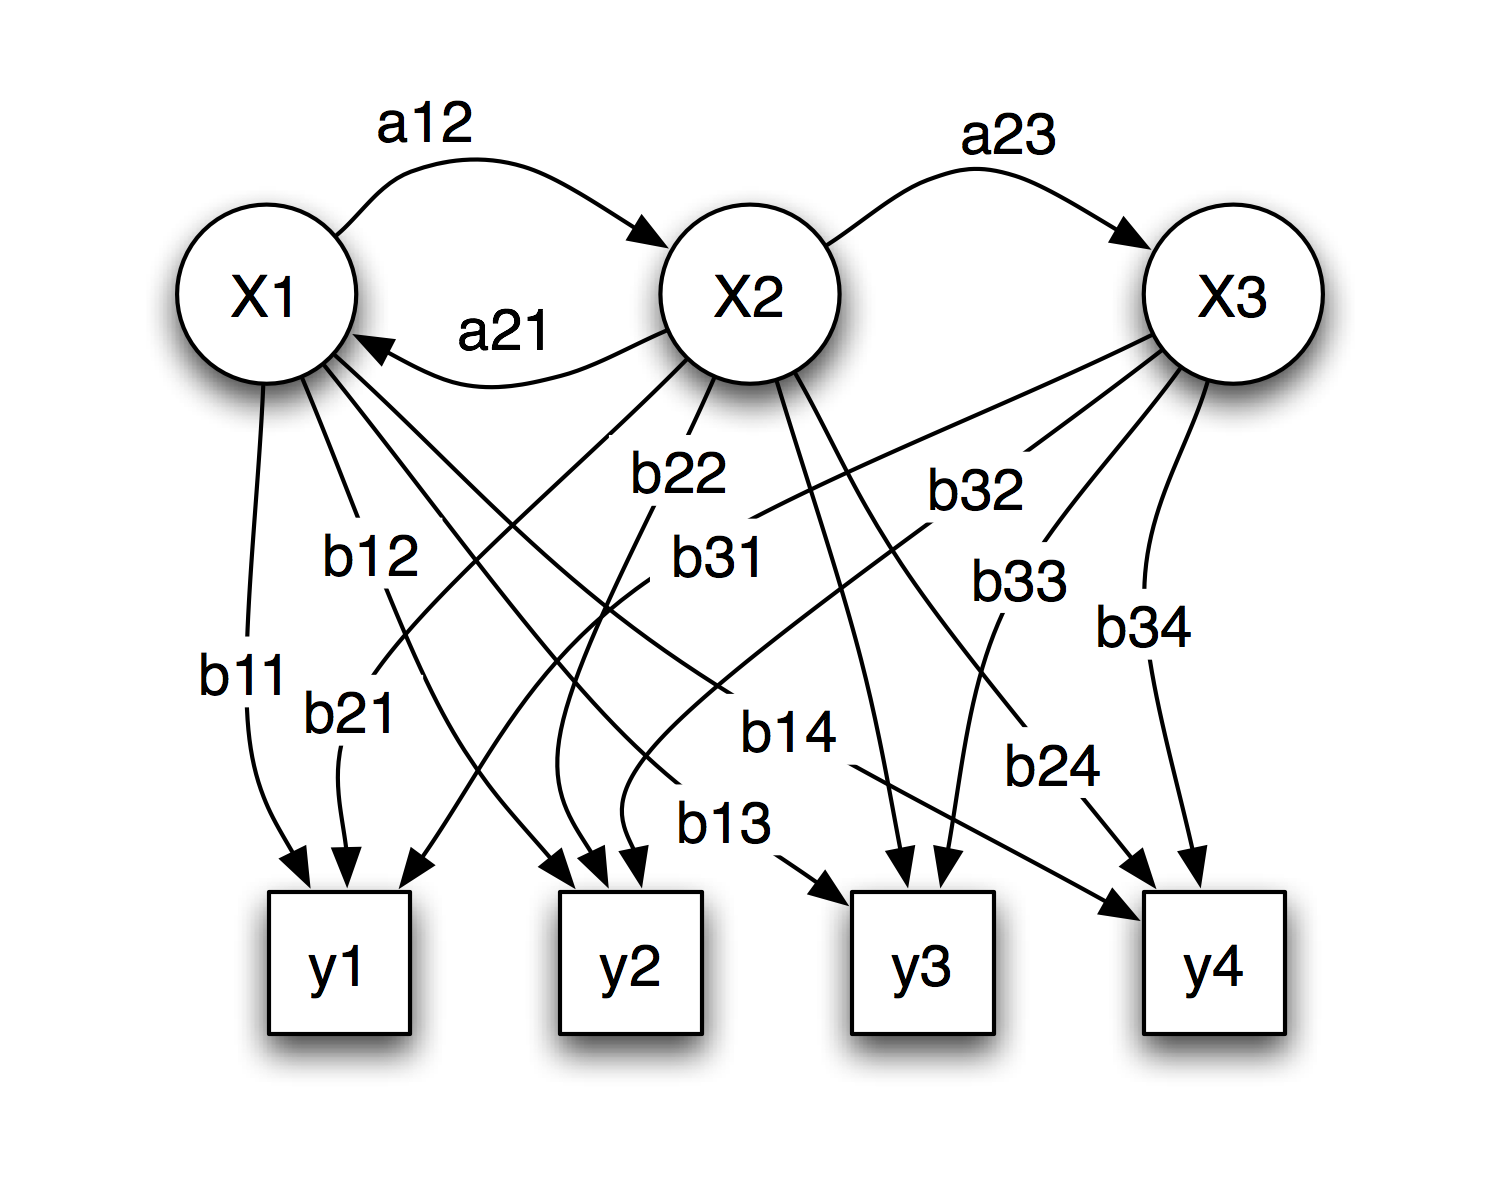
\includegraphics[height=150pt]{report5/hmm.png}
    \end{center}
    
\end{frame}

\begin{frame}{模型学习过程}
    \begin{enumerate}
        \item 为每一个词独立分配一个状态
        \item \textbf{\textcolor{red}{neighbor-merging(相邻合并}}
        \item 进一步合并
            \begin{itemize}
                \item V-merging
                \item M-merging
                \item Bayesian model merging
            \end{itemize}
    \end{enumerate}
\end{frame}


\begin{frame}{Neighbor-merging相邻合并}
    %Combines all states that share a transition and have the same class label.    
    合并有共同转移以及相同类别的所有状态
    \begin{center}
        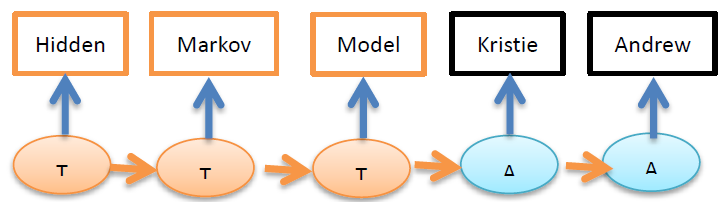
\includegraphics[width=250pt]{report5/neighbor-1.png}
    \end{center}
\end{frame}

\begin{frame}{Neighbor-merging相邻合并}
    %Combines all states that share a transition and have the same class label.    
    合并有共同转移以及相同类别的所有状态
    \begin{center}
        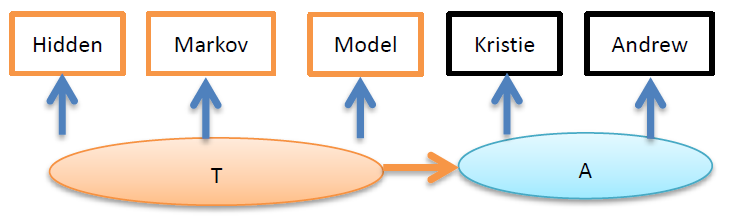
\includegraphics[width=250pt]{report5/neighbor-2.png}
    \end{center}
\end{frame}


\begin{frame}{模型学习过程}
    \begin{enumerate}
        \item 为每一个词独立分配一个状态
        \item neighbor-merging(相邻合并)
        \item 进一步合并
            \begin{itemize}
                \item \textbf{\textcolor{red}{V-merging}}
                \item M-merging
                \item Bayesian model merging
            \end{itemize}
    \end{enumerate}
\end{frame}



\begin{frame}{V-merging}
    合并任何有相同类别标签且转移到相同状态或者从共同状态转移的两个状态
    \begin{center}
        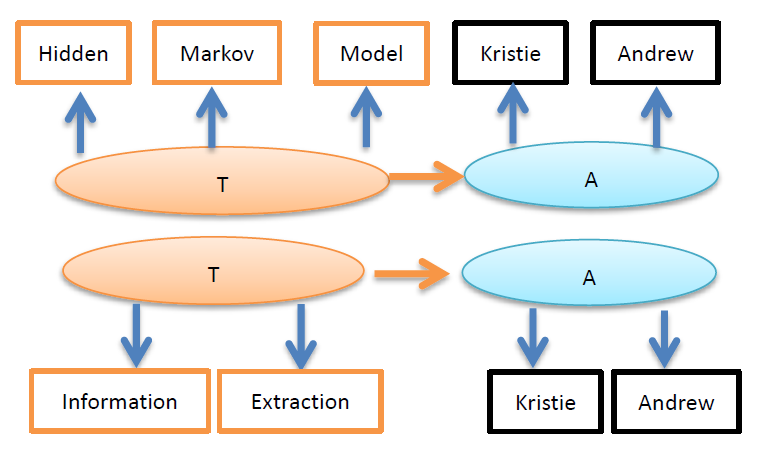
\includegraphics[height=150pt]{report5/v-merge-1.png}
    \end{center}
\end{frame}

\begin{frame}{V-merging}
    合并任何有相同类别标签且转移到相同状态或者从共同状态转移的两个状态
    \begin{center}
        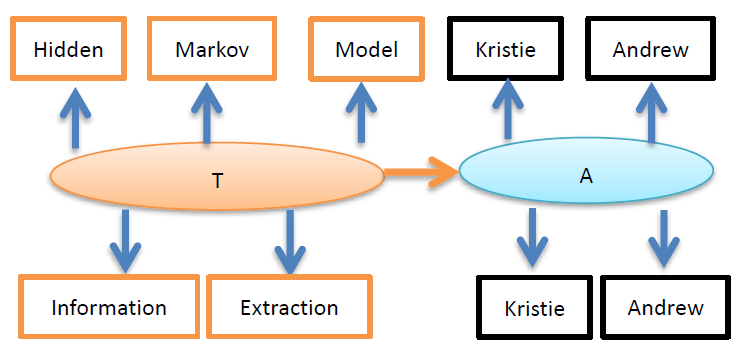
\includegraphics[height=120pt]{report5/v-merge-2.png}
    \end{center}
\end{frame}

\begin{frame}{模型学习过程}
    \begin{enumerate}
        \item 为每一个词独立分配一个状态
        \item neighbor-merging(相邻合并)
        \item 进一步合并
            \begin{itemize}
                \item V-merging
                \item \textbf{\textcolor{red}{M-merging}}
                \item \textbf{\textcolor{red}{Bayesian model merging}}
            \end{itemize}
    \end{enumerate}
\end{frame}


\begin{frame}{M-merging and Bayesian Model Merging}
\begin{block}{M-merging}
    
\end{block}

\begin{block}{Bayesian Model Merging}
    
\end{block}
\end{frame}



\section{实验结果}
\begin{frame}{Introduction}

\end{frame}

\section{Conclude}



\end{document}
